% !TEX encoding = UTF-8 Unicode
% !TEX root = ../report.tex
% 

\section{Construcción de la ontología}

\begin{figure}[h!]
  \makebox[\textwidth][c]{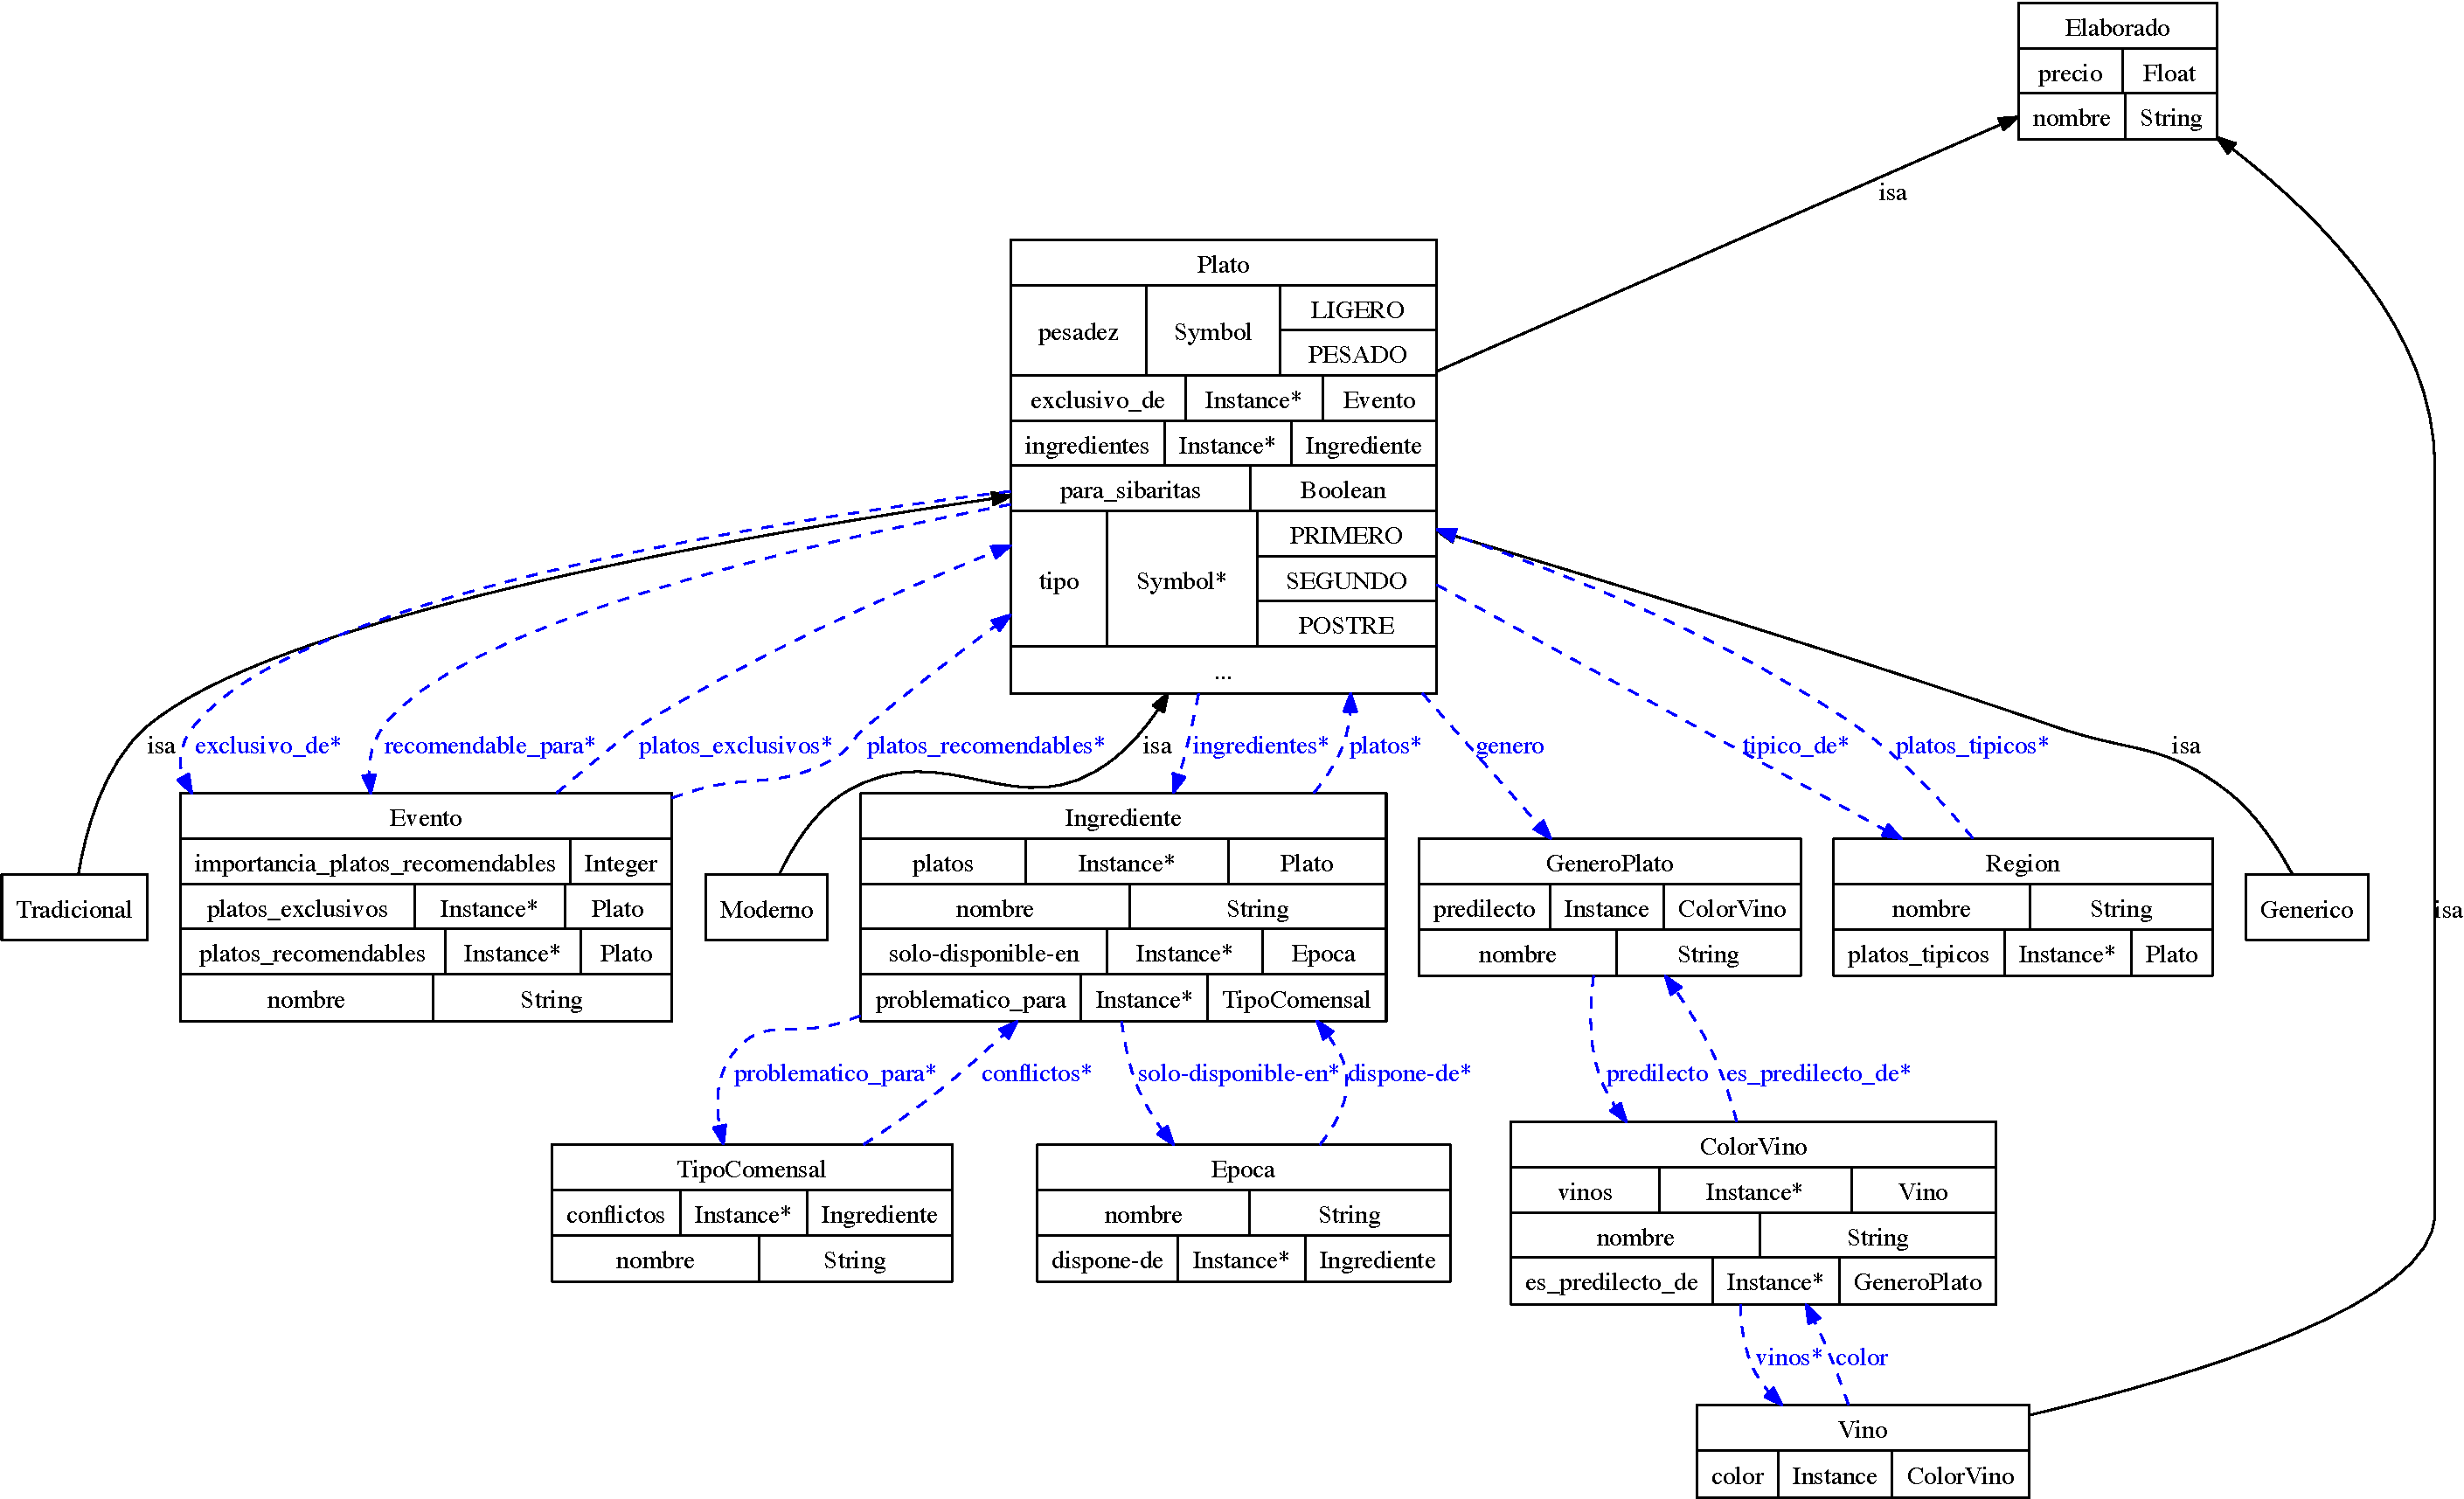
\includegraphics[width=1.2\textwidth]{%
      figures/ontologia}}
  \caption{La ontología final del problema}
\end{figure}

La construcción de la ontología (y de todo el sistema en general) se ha
realizado de manera iterativa, aunque inicialmente no había sido así.

En un principio habíamos construido sistema de clases completo pero incluso más
complejo de lo que ha sido finalmente, sin necesidad. Afortunadamente, esa
versión se perdió y empezamos con una más simple que solamente contenía las
clases elaborado, plato, bebida (que ahora es solamente vino) e ingrediente.

Luego añadimos la clase de tipos de comensal, para poder tener en cuenta
alergias y demás problemas alimenticios. También se añadió la clase época para
poder indicar la disponibilidad de ingredientes.

Inicialmente, los eventos iban a ser unos valores prefijados hasta que vimos
que podríamos sacarle más provecho a todo si eran instancias dentro de la
ontología. Así que creamos la clase evento y asociamos algunos platos como
preferidos en el evento. Para evitar que determinados platos propios de un
evento se recomendaran en otros donde no tuviera sentido (un claro ejemplo son
los pasteles de boda), casi al final hicimos la diferencia entre platos propios
y platos que son recomendables para los eventos.

Ya, más entrados en el proceso de implementación del sistema experto, añadimos
la clase región para poder modelar el origen geográfico/cultural de los
platos. Finalmente, cuando empezamos a tratar con los vinos, y tras considerar
que la bebida en general no tiene sentido para el problema que se nos pide
resolver, eliminamos la clase bebida, dejando solamente una clase para
vinos. Además, creamos la clase que modela el color del vino, que se asoció a
la nueva clase de géneros de plato (sopa, pescado, estofado, aperitivo, etc.)
para poder hacer la recomendación de vinos de manera más sencilla.

Fuera de aquí, también están las ontologías de solución del problema, que
solamente contienen las clases menú y menú abstracto. Más adelante detallaremos
su funcionamiento.

\subsection{Detalle de las clases de la ontología del problema}
\subsubsection{Clase \clase{Elaborado}}
Esta clase está construida para agrupar las características propias de los
productos que se venden con el menú: el \slot{nombre} y el
\slot{precio}. La idea es que cualquier cosa que esté en el menú debe ser un
producto elaborado.

En determinado momento tuvimos que hacer esta clase concreta para poder hacer
\emph{pattern matching} con CLIPS. Por suerte, los cambios que fuimos haciendo
en la implementación del problema provocaron que esta clase pudiera volver a
ser abstracta. Mientras la clase fue concreta, la clase \clase{Plato} también
tuvo que serlo porque CLIPS no permite subclases abstractas de clases
concretas.

\subsubsection{Clase \clase{Plato} y sus subclases}
La clase es abstracta y está dividida en las subclases \clase{Generico},
\clase{Moderno} y \clase{Tradicional}. Hemos decidido hacer esta clasificación
porque no es habitual que un plato sea moderno y tradicional a la vez, y
también existen platos que no se considerarían tradicionales pero que son
platos que se consumen habitualmente (de ahí el término genérico).

Además del nombre y el precio derivados de \clase{Elaborado}, la clase
\clase{Plato} proporciona nuevos campos:
\begin{slotlist}
\item[ingredientes] Es un campo múltiple de instancias de la clase
  \clase{Ingrediente}. Es necesario que haya como mínimo un ingrediente.
\item[genero] Es un campo simple que apunta a una instancia de
  \clase{GeneroPlato}. Sirve para clasificar los platos en sus géneros.
\item[tipo] Un campo múltiple que indica si el plato es \emph{primero},
  \emph{segundo} o \emph{postre}. Es necesario que sea algún tipo de plato.
\item[para\_sibaritas] Un campo cierto/falso. Los platos para sibaritas no
  queremos que se recomienden a alguien que no lo es, pues es habitual que no
  lo quieran. Por otro lado, se les da prioridad si el cliente sí lo es.
\item[temperatura] Indica si el plato es frío o caliente.
\item[pesadez] Indica si un plato es ligero o pesado. En general, no es bueno
  que un cliente coma dos platos ligeros o dos platos pesados.
\item[tipico\_de] Es un campo múltiple que contiene las instancias de
  \clase{Region} de donde es típico el plato, si es el caso.
\item[recomendable\_para] Un campo múltiple que contiene, si es el caso, en qué
  eventos pueden preferir el plato, para que se priorice.
\item[exclusivo\_de] A diferencia del anterior, si está definido indica en qué
  eventos puede ofrecerse el plato de forma exclusiva (por ejemplo, un pastel
  de boda solamente puede ofrecerse en una boda). También lo prioriza.
\item[dificultad] Indica, mediante un valor de 0 a 100, la dificultad de
  elaboración del plato (un valor mayor indica una dificultad mayor). Cuantos
  más comensales hay en la celebración, más importante es que el plato sea más
  sencillo de elaborar.
\end{slotlist}

Las subclases de \clase{Plato} no contienen ningún slot propio. Simplemente es
para poder separar correctamente y poder hacer uso del \emph{pattern matching}
en CLIPS.

\subsubsection{Clase \clase{GeneroPlato}}
Mediante esta clase se modelan los distintos géneros de plato en función de
cómo son. Es decir, sopas, platos de pescado, estofados, etc. Se utiliza para
poder agrupar platos similares que precisan vinos de colores similares. Por
tanto, además del \slot{nombre} del género, el único campo que tienen es
\slot{predilecto}, que apunta al color de vino más acorde con los platos de ese
género.

No tienen el campo inverso hacia \clase{Plato} con los platos del género porque
no lo usamos durante el problema.

\subsubsection{Clase \clase{Vino}}
Esta clase representa a los vinos. Además de los campos de \clase{Elaborado},
contiene un campo \slot{color} que apunta a la instancia de \clase{ColorVino}
con el color del vino.

\subsubsection{Clase \clase{ColorVino}}
Como ya hemos comentado con anterioridad, esta clase representa los colores que
puede tomar un vino. Los campos que tiene, además del \slot{nombre} del color,
son dos:
\begin{slotlist}
\item[es\_predilecto\_de] Es el campo múltiple que contiene la lista de géneros
  de plato que prefieren ese color de vino. Por tanto, es el inverso del campo
  \clase{Vino}:\slot{predilecto}.
\item[vinos] Este campo múltiple guarda la lista de vinos del color. Es el
  campo inverso de \clase{Vino}+:\slot{color}.
\end{slotlist}

\subsubsection{Clase \clase{Ingrediente}}
Como todas las clases que hay en la ontología, esta clase tiene el campo
\slot{nombre} para identificar a sus instancias. En este caso, además, están
los campos siguientes:
\begin{slotlist}
\item[platos] Este campo múltiple contiene los platos que utilizan el
  ingrediente en su elaboración. Es el campo inverso de
  \clase{Plato}:\slot{ingredientes}.
\item[problematico\_para] Es un campo múltiple con las instancias de
  \clase{Tipo} Comensal+ que no pueden consumir el ingrediente. Muy importante
  para modelar las alergias y restricciones culturales de la comida.
\item[solo-disponible-en] Cuando está definido, este campo múltiple contiene
  las instancias de \clase{Epoca} en las que el ingrediente está disponible para
  elaborar platos. Si no tiene ninguna indicación es que el ingrediente se
  puede usar todo el año.
\end{slotlist}

\subsubsection{Clase \clase{Region}}
En este caso, la clase la utilizamos para tener constancia de las zonas
geográficas. Con ello, podemos saber el origen de un plato. Además del
\slot{nombre}, el campo que contiene es \slot{platos\_tipicos}, con todos los
platos típicos de la región y que es el inverso de
\clase{Plato}:\slot{tipico\_de}.

\subsubsection{Clase \clase{Epoca}}
Los ingredientes, como ya hemos visto, no están disponibles durante todo el año
necesariamente. Esta clase tiene como instancias las cuatro estaciones del año,
cada una con su \slot{nombre} y el campo múltiple \slot{dispone-de} con la
lista de ingredientes disponibles durante la época (en el caso de los
ingredientes anuales, no aparecen). Este segundo campo es, entonces, el inverso
de \clase{Ingrediente}:\slot{solo-disponible-en}

\subsubsection{Clase \clase{Evento}}
La clase \clase{Evento} contiene las instancias que representan los posibles
eventos para los que el catering puede ofrecer menús especiales. Además del
\slot{nombre} que identifica el evento, la clase contiene otros campos:
\begin{slotlist}
\item[platos\_exclusivos] Este campo múltiple, inverso de
  \clase{Plato}:\slot{exclusivo\_de} contiene los platos que son exclusivos
  para las celebraciones del evento en cuestión.
\item[platos\_recomendables] De forma similar al anterior, es el inverso de
  \clase{Plato}:\slot{recomendable\_para} y contiene los platos que son
  recomendables para las celebraciones del evento.
\item[importancia\_platos\_recomendables] Este es un campo numérico que indica
  cuán importante es que se incluya un plato recomendable dentro de las
  propuestas de menú. En el caso de los exclusivos no se usa esta ponderación
  porque se supone que en esos casos es casi necesario que estén.
\end{slotlist}

\subsubsection{Clase \clase{TipoComensal}}
Hay una serie de comensales, especialmente los alérgicos (celíacos, alergias a
huevo, leche), vegetarianos, y demás que precisan unos platos especiales que no
tengan determinados ingredientes. Para estos casos está la clase
\clase{TipoComensal}, que además del \slot{nombre} del tipo contiene el campo
\slot{conflictos} con toda la lista de ingredientes que no son compatibles con
el tipo de comensal. Este campo es el inverso de
\clase{Ingrediente}:\slot{problematico\_para}.

\subsection{Detalle de las clases de la ontología de la solución}
\begin{figure}[h]
  \makebox[\textwidth][c]{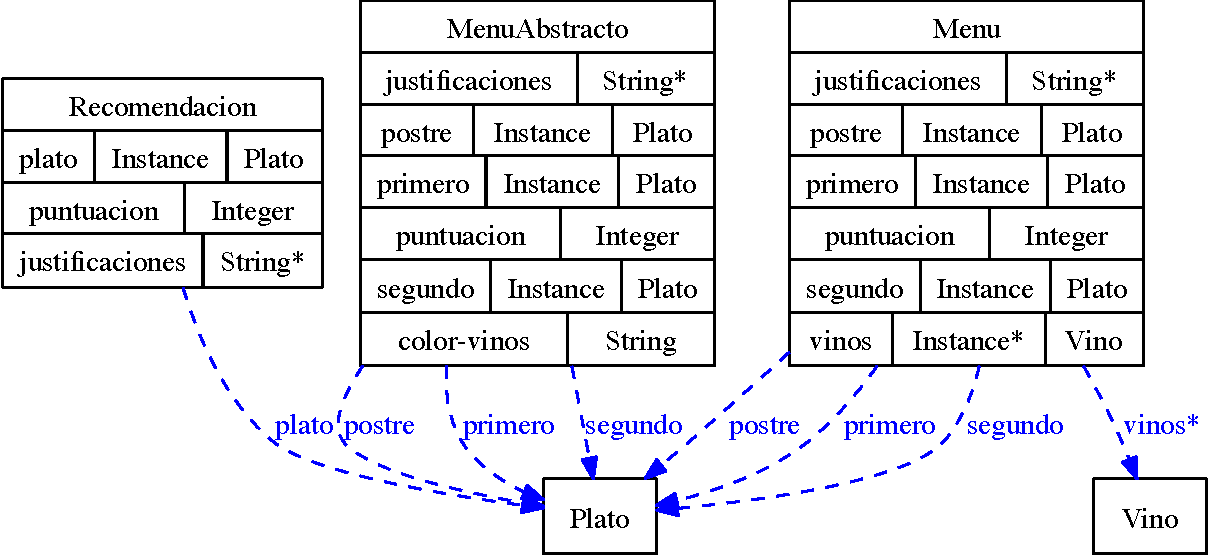
\includegraphics[width=0.7\textwidth]{%
      figures/ontologia-solucion}}
  \caption{La ontología de la solución}\label{ont:solucion}
\end{figure}

Estas clases no las hemos construido con Protégé, sino que las hemos definido a
mano en el sistema mediante la construcción \verb+defclass+ porque todas sus
instancias las genera el sistema. Igualmente, en la figura \ref{ont:solucion}
puede verse el esquema que sigue la ontología.

\subsubsection{Clase \clase{Recomendacion}}
Esta clase representa la recomendación de un plato, elaborada con los datos de
entrada del usuario y el conocimiento propio del sistema. Los campos que
contiene son:
\begin{slotlist}
\item[plato] La instancia de \clase{Plato} (de la ontología del problema) sobre
  la que trata la recomendación.
\item[justificaciones] Contiene la lista de justificaciones (con sus
  puntuciones individuales) para la puntuación que recibe el plato.
\item[puntuacion] Es el valor numérico (entero) con la valoración de la
  recomendación.
\end{slotlist}

\subsubsection{Clases \clase{MenuAbstracto} y \clase{Menu}}
Son dos clases muy similares que se corresponden con las soluciones al
problema. Los campos que tienen en común son:
\begin{slotlist}
\item[primero] La instancia de \clase{Recomendacion} que representa al primer
  plato.
\item[segundo] La instancia de \clase{Recomendacion} que representa al segundo
  plato.
\item[postre] La instancia de \clase{Recomendacion} que representa al postre.
\item[justificaciones] Las justificaciones para la puntuación del menú. Una de
  ellas indica, simplemente, los puntos que suman sus platos.
\item[puntuacion] El valor numérico con la valoración del menú.
\end{slotlist}

Además, \clase{MenuAbstracto} contiene un campo múltiple de cadenas
(\emph{strings}) llamado \slot{colores-vino} con los colores de vino que se
admiten. Si tiene más de un valor (como máximo dos), el primero es para el
primer plato y el segundo para el segundo.

En el caso de \clase{Menu}, contiene el campo múltiple \slot{vinos} con las
instancias de \clase{Vino} que se sirven con el menú. Si hay dos valores, el
primero es para el primer plato y el segundo para el segundo.
